\documentclass[border=5pt]{standalone}
\usepackage{fontspec,xeCJK,amsmath,amssymb,tikz,graphicx}
\usetikzlibrary{arrows.meta,calc}
\setmainfont{Arial}\setCJKmainfont{PingFang SC}
\definecolor{ink}{HTML}{203340}\definecolor{blue}{HTML}{147E91}\definecolor{pale}{HTML}{EEF6F6}\definecolor{warm}{HTML}{AE651E}\definecolor{cream}{HTML}{FFF6E9}\definecolor{line}{HTML}{CFDDDF}
% All illustrations are retained unmodified from the built-in imagegen draft.
% Crop scopes set scale by total image width, avoiding image DPI assumptions.
\newcommand{\tile}[3]{\begin{tikzpicture}\clip(0,0)rectangle(2,2);\node[anchor=north west,inner sep=0] at (#1,#2){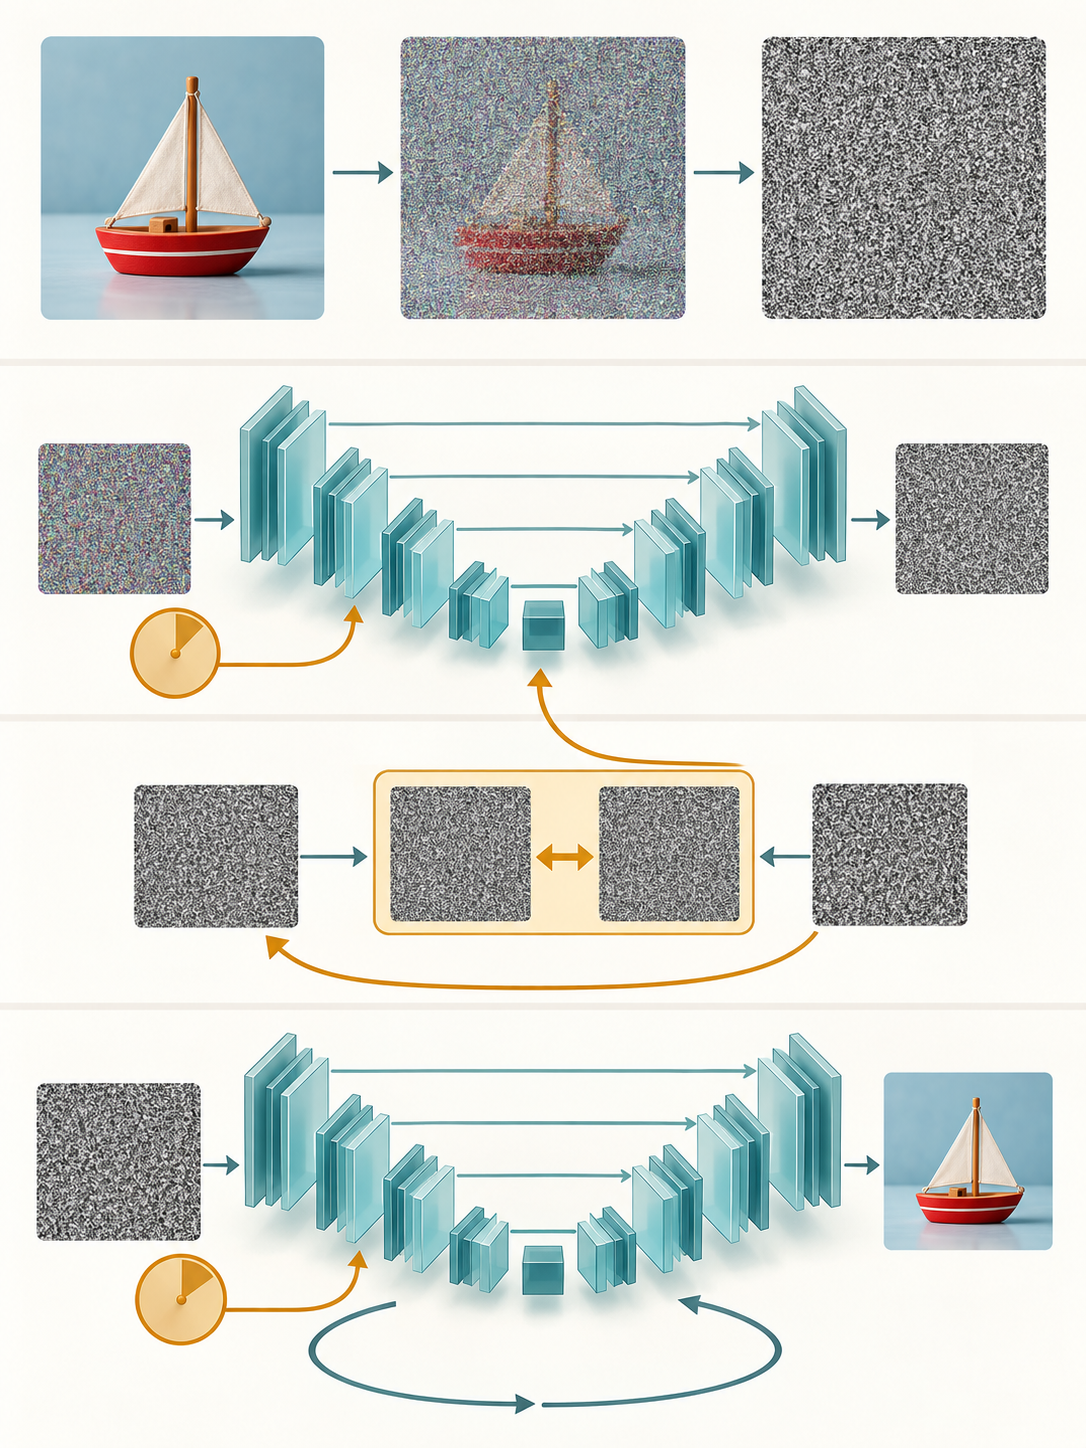
\includegraphics[width=#3cm]{ddpm-imagegen-draft.png}};\end{tikzpicture}}
\begin{document}
\begin{tikzpicture}[x=1cm,y=1cm,every node/.style={text=ink,font=\fontsize{10}{13}\selectfont},flow/.style={-{Stealth[length=5pt]},draw=blue,line width=1pt},update/.style={-{Stealth[length=5pt]},draw=warm,dashed,line width=1pt},box/.style={rounded corners=5pt,draw=line,fill=white}]
\path[use as bounding box](0,0)rectangle(10.5,30.5);\fill[pale](0,0)rectangle(10.5,30.5);
\node[font=\fontsize{20}{24}\selectfont\bfseries] at(5.25,29.8){DDPM：只预测噪声，如何生成？};
\node[text=blue]at(5.25,29.15){训练：随机抽一题　｜　生成：倒着走完 1000 步};
\draw[box](.35,23.1)rectangle(10.15,28.65);
\node[anchor=west,font=\fontsize{13}{16}\selectfont\bfseries]at(.65,28.15){A　造训练题｜固定前向过程};
\node at(1.95,26.3){\tile{-.28}{2.25}{7.5}};
\node at(5.25,26.3){\tile{-2.76}{2.25}{7.5}};
\node at(8.55,26.3){\tile{-5.26}{2.25}{7.5}};
\draw[flow](3.05,26.3)--(4.12,26.3);\draw[flow](6.35,26.3)--(7.42,26.3);
\node at(1.95,24.92){干净图 $x_0$};\node at(5.25,24.92){噪声图 $x_t$};\node at(8.55,24.92){接近纯噪声 $x_T$};
\node at(5.25,24.25){$x_t=\sqrt{\bar\alpha_t}\,x_0+\sqrt{1-\bar\alpha_t}\,\epsilon$};
\node[font=\fontsize{9}{12}\selectfont]at(5.25,23.55){$x_0,x_t,\epsilon:\ H\!\times\!W\!\times\!3$；随机抽 $t$，直接算 $x_t$};
\draw[flow](5.25,23.1)--(5.25,22.65);
\draw[box](.35,14.5)rectangle(10.15,22.65);
\node[anchor=west,font=\fontsize{13}{16}\selectfont\bfseries]at(.65,22.15){B　同一个 U-Net｜$\epsilon_\theta(x_t,t)$};
% Retain the complete model illustration only, no draft arrows or time dial.
\begin{scope}\clip(1.8,18.15)rectangle(8.7,21.45);\node[anchor=north west,inner sep=0]at(-.75,25.6){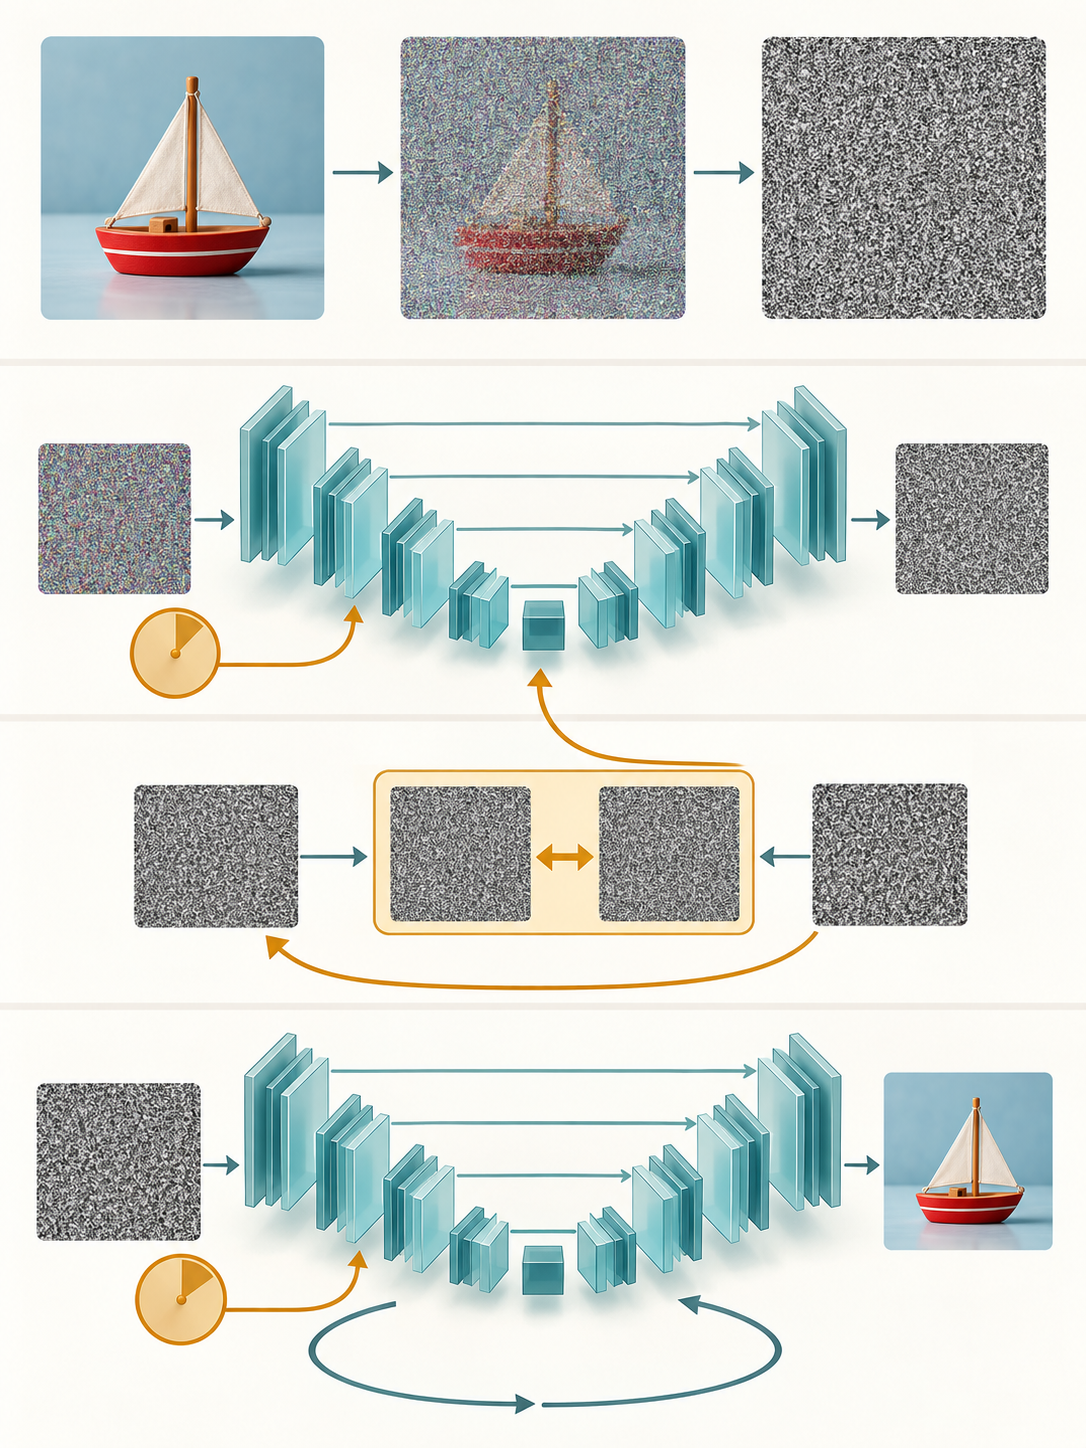
\includegraphics[width=12cm]{ddpm-imagegen-draft.png}};\end{scope}
\node[fill=white,inner sep=3pt]at(5.25,17.65){32$^2$ 模型分辨率：$32\to16\to8\to4\to8\to16\to32$};
\node at(5.25,16.95){$t\to$ 正弦时间嵌入 $\to$ 各残差块};
\node at(5.25,16.35){16$\times$16 自注意力；GroupNorm；跨时间共享参数 $\theta$};
\node at(5.25,15.72){输出 $\hat\epsilon=\epsilon_\theta(x_t,t)$，形状仍为 $H\times W\times3$};
\node[font=\fontsize{9}{12}\selectfont,text=blue]at(5.25,15.05){训练与采样都调用此网络；采样时参数固定};
\draw[flow](5.25,14.5)--(5.25,14.05);
\draw[box,fill=cream](.35,10.2)rectangle(10.15,14.05);
\node[anchor=west,font=\fontsize{13}{16}\selectfont\bfseries]at(.65,13.55){C　训练｜答案是亲手加进去的 $\epsilon$};
\node at(5.25,12.75){$L_{\rm simple}=\mathbb E\lVert\epsilon-\epsilon_\theta(x_t,t)\rVert_2^2$};
\node at(5.25,11.95){真实噪声 $\epsilon$ 对照预测 $\hat\epsilon$；梯度只更新 $\theta$};
\node[font=\fontsize{9}{12}\selectfont]at(5.25,11.2){抽数据 $\to$ 抽 $t$ $\to$ 加噪 $\to$ 预测 $\to$ 算误差 $\to$ 更新};
\node[font=\fontsize{9}{12}\selectfont,text=warm]at(5.25,10.65){一次训练迭代无需展开全部 1000 次反向去噪};
\draw[update](.65,12.1)--(.05,12.1)--(.05,16.7)--(.35,16.7);
\draw[box](.35,2.6)rectangle(10.15,9.65);
\node[anchor=west,font=\fontsize{13}{16}\selectfont\bfseries]at(.65,9.15){D　生成｜从 $x_T\sim\mathcal N(0,I)$ 开始};
\node at(1.85,7.55){\tile{-5.26}{2.25}{7.5}};
\node at(8.6,7.55){\tile{-.28}{2.25}{7.5}};
\node[draw=line,rounded corners=3pt,fill=pale,minimum width=2.8cm,minimum height=1cm]at(5.2,7.55){反复调用 B};
\draw[flow](2.9,7.55)--(3.8,7.55);\draw[flow](6.6,7.55)--(7.5,7.55);
\node at(5.25,6.05){$\displaystyle\mu_\theta=\frac{x_t-\frac{\beta_t}{\sqrt{1-\bar\alpha_t}}\,\epsilon_\theta(x_t,t)}{\sqrt{\alpha_t}}$};
\node at(5.25,4.95){$x_{t-1}=\mu_\theta+\sigma_t z$；$t=1000,\ldots,1$};
\node[font=\fontsize{9}{12}\selectfont]at(5.25,4.2){$z\sim\mathcal N(0,I)$；最后一步 $z=0$；固定 $\sigma_t^2=\beta_t$ 或 $\tilde\beta_t$};
\node[font=\fontsize{9}{12}\selectfont,text=blue]at(5.25,3.4){$x_{t-1}$ 回到 B，时间减 1；到 $t=1$ 后返回图像};
\draw[flow](9.85,5.05)--(10.38,5.05)--(10.38,8.5)--(5.2,8.5)--(5.2,8.05);
\node[font=\fontsize{11}{14}\selectfont\bfseries]at(5.25,1.8){E　检验｜画得好、算得像、生成快，分别看};
\node[font=\fontsize{9}{12}\selectfont]at(5.25,1.15){Table 1/2：质量与消融　Fig. 5--8：压缩、分支与插值};
\node[font=\fontsize{9}{12}\selectfont]at(5.25,.55){读图路线：§2 看 A；§3 看 B/C/D；§4 看 E；§5--6 回看整条链};
\end{tikzpicture}\end{document}
